% Fig 3 — RTL module-level dataflow (hardware wiring with named ports)
% Shows physical modules and the named wires connecting them.
% Compile:  pdflatex fig3_dataflow.tex
\documentclass[tikz,border=6pt]{standalone}
\usepackage{xcolor}
\usetikzlibrary{positioning, shapes.geometric, arrows.meta, fit, calc,
                shadows.blur, backgrounds}

\definecolor{ctrlclr}{RGB}{255,225,225}
\definecolor{memclr} {RGB}{218,205,250}
\definecolor{peclr}  {RGB}{215,240,215}
\definecolor{lutclr} {RGB}{255,240,200}
\definecolor{wirelbl}{RGB}{60,60,60}

\begin{document}
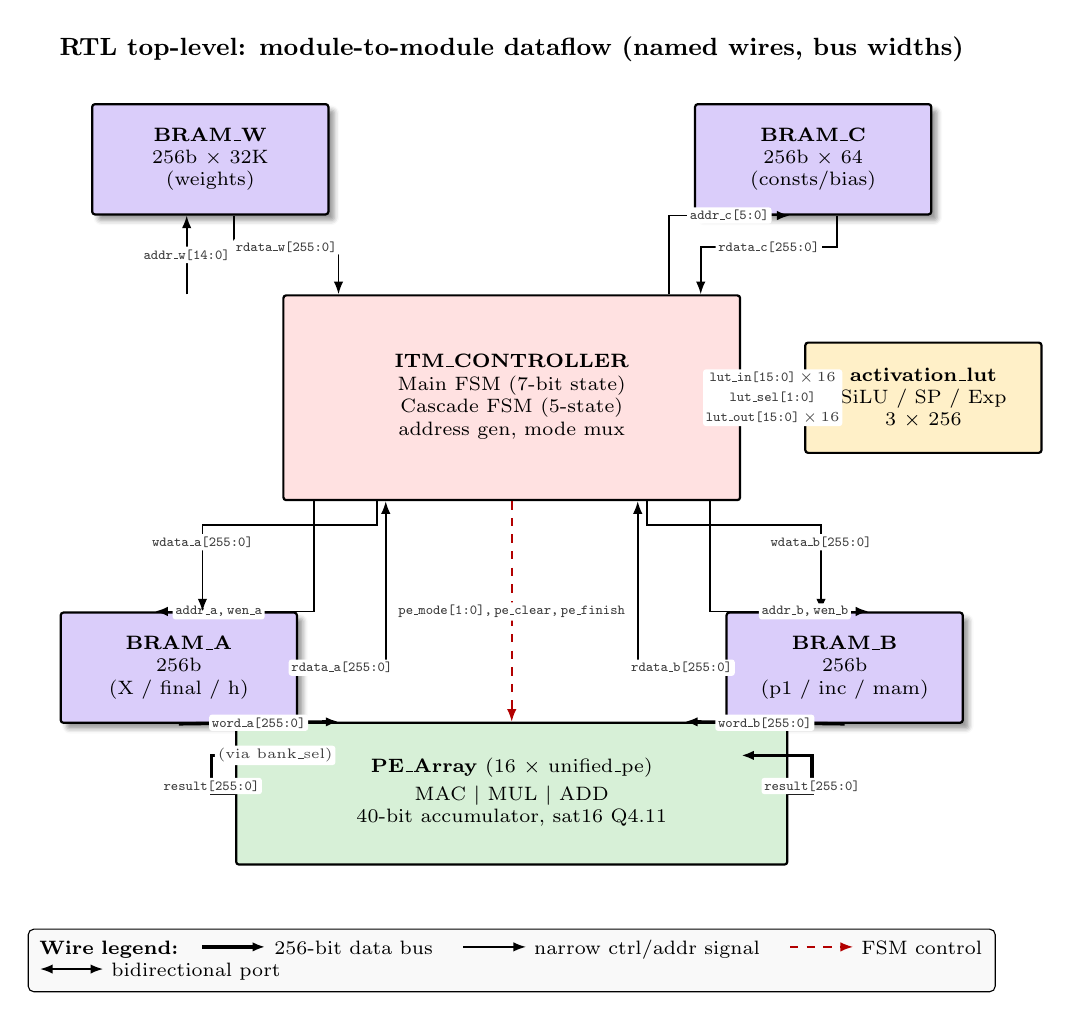
\begin{tikzpicture}[
    font=\scriptsize,
    >={Latex[length=1.6mm]},
    % Module box — Verilog "module foo" with ports
    mod/.style    ={draw, thick, rounded corners=1pt, align=center,
                    minimum width=30mm, minimum height=14mm,
                    inner sep=3pt, fill=white},
    ctrl/.style   ={mod, fill=ctrlclr, minimum width=58mm, minimum height=26mm},
    mem/.style    ={mod, fill=memclr, blur shadow={shadow blur steps=4}},
    pe/.style     ={mod, fill=peclr,  minimum width=70mm, minimum height=18mm},
    lut/.style    ={mod, fill=lutclr},
    % Wires
    wire/.style   ={->, semithick},
    wirebi/.style ={<->, semithick},
    bus/.style    ={->, line width=1.2pt},
    busbi/.style  ={<->, line width=1.2pt},
    wlbl/.style   ={font=\tiny, color=wirelbl, inner sep=1pt,
                    fill=white, rounded corners=1pt},
    port/.style   ={font=\tiny, color=black!70, inner sep=1pt},
]

% =================== ITM_CONTROLLER (central) ===================
\node[ctrl] (ctrl) at (0,0)
    {\textbf{ITM\_CONTROLLER}\\[2pt]
     \begin{tabular}{c}
       Main FSM (7-bit state)\\
       Cascade FSM (5-state)\\
       address gen, mode mux
     \end{tabular}};

% =================== BRAMs (top row) ===================
\node[mem, above left=10mm and -6mm of ctrl]  (rW) {\textbf{BRAM\_W}\\ \scriptsize 256b $\times$ 32K\\ \scriptsize (weights)};
\node[mem, above right=10mm and -6mm of ctrl] (rC) {\textbf{BRAM\_C}\\ \scriptsize 256b $\times$ 64\\ \scriptsize (consts/bias)};

% =================== BRAMs (left/right of PE Array) ===================
\node[mem, below left =14mm and -2mm of ctrl] (rA) {\textbf{BRAM\_A}\\ \scriptsize 256b\\ \scriptsize (X / final / h)};
\node[mem, below right=14mm and -2mm of ctrl] (rB) {\textbf{BRAM\_B}\\ \scriptsize 256b\\ \scriptsize (p1 / inc / mam)};

% =================== PE_Array (bottom) ===================
\node[pe, below=28mm of ctrl] (pe)
    {\textbf{PE\_Array} (16 $\times$ unified\_pe)\\[2pt]
     \begin{tabular}{c}
       MAC $|$ MUL $|$ ADD\\
       40-bit accumulator, sat16 Q4.11
     \end{tabular}};

% =================== Activation LUT (right) ===================
\node[lut, right=8mm of ctrl] (lut) {\textbf{activation\_lut}\\ \scriptsize SiLU / SP / Exp\\ \scriptsize 3 $\times$ 256};

% =================== Wires: Controller <-> BRAM_W ===================
\draw[wire]   (ctrl.north -| rW.south)
              ++(-3mm,0) coordinate (cw1) -- ($(rW.south)+(-3mm,0)$)
              node[wlbl, midway]{\texttt{addr\_w[14:0]}};
\draw[wire]   ($(rW.south)+(3mm,0)$) -- ++(0,-4mm) -| ($(ctrl.north)+(-22mm,0)$)
              node[wlbl, pos=0.25]{\texttt{rdata\_w[255:0]}};

% =================== Wires: Controller <-> BRAM_C ===================
\draw[wire]   ($(ctrl.north)+(20mm,0)$) |- ($(rC.south)+(-3mm,0)$)
              node[wlbl, pos=0.75]{\texttt{addr\_c[5:0]}};
\draw[wire]   ($(rC.south)+(3mm,0)$) -- ++(0,-4mm) -| ($(ctrl.north)+(24mm,0)$)
              node[wlbl, pos=0.25]{\texttt{rdata\_c[255:0]}};

% =================== Wires: Controller <-> BRAM_A ===================
% addr + wen + wdata going down
\draw[wire]   ($(ctrl.south west)+(4mm,0)$) |- ($(rA.north)+(-3mm,0)$)
              node[wlbl, pos=0.8]{\texttt{addr\_a,\,wen\_a}};
\draw[wire]   ($(ctrl.south west)+(12mm,0)$) -- ++(0,-3mm) -| ($(rA.north)+(3mm,0)$)
              node[wlbl, pos=0.6]{\texttt{wdata\_a[255:0]}};
% rdata coming back up
\draw[wire]   (rA.east) -| ($(ctrl.south)+(-16mm,0)$)
              node[wlbl, pos=0.25]{\texttt{rdata\_a[255:0]}};

% =================== Wires: Controller <-> BRAM_B ===================
\draw[wire]   ($(ctrl.south east)+(-12mm,0)$) -- ++(0,-3mm) -| ($(rB.north)+(-3mm,0)$)
              node[wlbl, pos=0.6]{\texttt{wdata\_b[255:0]}};
\draw[wire]   ($(ctrl.south east)+(-4mm,0)$) |- ($(rB.north)+(3mm,0)$)
              node[wlbl, pos=0.8]{\texttt{addr\_b,\,wen\_b}};
\draw[wire]   (rB.west) -| ($(ctrl.south)+(16mm,0)$)
              node[wlbl, pos=0.25]{\texttt{rdata\_b[255:0]}};

% =================== Wires: BRAM_A/B -> PE_Array (operands) ===================
\draw[bus]    (rA.south) -- ($(pe.north)+(-22mm,0)$)
              node[wlbl, pos=0.5]{\texttt{word\_a[255:0]}};
\draw[bus]    (rB.south) -- ($(pe.north)+(22mm,0)$)
              node[wlbl, pos=0.5]{\texttt{word\_b[255:0]}};

% =================== Wires: Controller -> PE_Array (control) ===================
\draw[wire, dashed, red!70!black]
              (ctrl.south) -- ($(pe.north)+(0,0)$)
              node[wlbl, pos=0.5]
              {\texttt{pe\_mode[1:0],\,pe\_clear,\,pe\_finish}};

% =================== Wires: PE_Array -> BRAM_A/B (result writeback) ===================
\draw[bus]    (pe.west) -- ++(-3mm,0) |- ($(rA.south east)+(-2mm,-4mm)$)
              node[wlbl, pos=0.1]{\texttt{result[255:0]}}
              node[wlbl, pos=0.95]{(via bank\_sel)};
\draw[bus]    (pe.east) -- ++(3mm,0) |- ($(rB.south west)+(2mm,-4mm)$)
              node[wlbl, pos=0.1]{\texttt{result[255:0]}};

% =================== Wires: Controller <-> LUT ===================
\draw[wirebi] (ctrl.east) -- (lut.west)
              node[wlbl, pos=0.5]
              {\shortstack{\texttt{lut\_in[15:0]}\,$\times$\,16\\
                           \texttt{lut\_sel[1:0]}\\
                           \texttt{lut\_out[15:0]}\,$\times$\,16}};

% =================== Legend ===================
\node[draw, rounded corners=2pt, fill=gray!5, align=left,
      below=8mm of pe, font=\scriptsize, text width=120mm, inner sep=4pt] (lg)
    {\textbf{Wire legend:}\quad
     \tikz[baseline]\draw[bus](0,1mm)--(8mm,1mm); 256-bit data bus  \quad
     \tikz[baseline]\draw[wire](0,1mm)--(8mm,1mm); narrow ctrl/addr signal  \quad
     \tikz[baseline]\draw[wire,dashed,red!70!black](0,1mm)--(8mm,1mm); FSM control  \quad
     \tikz[baseline]\draw[wirebi](0,1mm)--(8mm,1mm); bidirectional port};

% =================== Title ===================
\node[font=\bfseries\small, above=4mm of rW.north -| ctrl.north] (ttl)
    {RTL top-level: module-to-module dataflow (named wires, bus widths)};

\end{tikzpicture}
\end{document}
